\documentclass[12pt, twoside]{article}
\input{../preamble}
\usepackage{pgfplots}
\pgfplotsset{compat=1.18}

\fancyhead[LE]{\thepage}
\fancyhead[RO]{Markscheme}
\fancyhead[LO]{La Scuola d'Italia / Dr.\ Huson / IB Math \\* 15 April 2026}

\begin{document}
\subsubsection*{6.6 Classwork: The Discriminant and Polynomial Equations (no calculator) --- Markscheme}

\begin{enumerate}[itemsep=0.15cm]

%--- Problem 1: Discriminant basics [5 marks] ---
\item[1.] [Maximum mark: 5]

For each quadratic function, find the discriminant $\Delta = b^2 - 4ac$
and state the number of real roots.

\begin{enumerate}[itemsep=0.3cm]
  \item $f(x) = x^2 - 6x + 9$

  $\Delta = (-6)^2 - 4(1)(9) = 36 - 36 = 0$ \hfill \textbf{(A1)}

  One repeated real root (the parabola touches the $x$-axis). \hfill \textbf{(A1)}

  \item $g(x) = 2x^2 + 3x + 5$

  $\Delta = 3^2 - 4(2)(5) = 9 - 40 = -31$ \hfill \textbf{(A1)}

  No real roots ($\Delta < 0$; the parabola does not cross the $x$-axis). \hfill \textbf{(A1)}

  \item $\Delta = 0$: graph touches the $x$-axis at one point (repeated root).
  $\Delta < 0$: graph does not intersect the $x$-axis. \hfill \textbf{(A1)}
\end{enumerate}

%--- Problem 2: Discriminant with parameter [6 marks] ---
\item[2.] [Maximum mark: 6]

The equation $x^2 + kx + 9 = 0$ has two equal roots.

\begin{enumerate}[itemsep=0.3cm]
  \item $\Delta = k^2 - 4(1)(9) = k^2 - 36$ \hfill \textbf{(A1)}

  \item For equal roots, $\Delta = 0$: \hfill \textbf{(M1)}

  $k^2 - 36 = 0 \implies k^2 = 36 \implies k = \pm 6$ \hfill \textbf{(A1)}

  \item When $k = 6$: $x^2 + 6x + 9 = (x + 3)^2 = 0$, so $x = -3$. \hfill \textbf{(A1)}

  When $k = -6$: $x^2 - 6x + 9 = (x - 3)^2 = 0$, so $x = 3$. \hfill \textbf{(A1)}

  \item No real roots when $\Delta < 0$: $k^2 - 36 < 0$, i.e.\ $-6 < k < 6$. \hfill \textbf{(A1)}
\end{enumerate}

\newpage

%--- Problem 3: Line tangent to parabola [7 marks] ---
\item[3.] [Maximum mark: 7]

The line $y = 2x + c$ is tangent to the parabola $y = x^2 + 1$.

\begin{enumerate}[itemsep=0.3cm]
  \item Setting equal: $x^2 + 1 = 2x + c$

  $x^2 - 2x + 1 - c = 0$, i.e.\ $x^2 - 2x + (1 - c) = 0$ \hfill \textbf{(AG)}

  \item $\Delta = (-2)^2 - 4(1)(1 - c) = 4 - 4 + 4c = 4c$ \hfill \textbf{(M1)}

  For tangency: $\Delta = 0 \implies 4c = 0 \implies c = 0$ \hfill \textbf{(A1)}

  \item With $c = 0$: $x^2 - 2x + 1 = 0 \implies (x - 1)^2 = 0$,
  so $x = 1$. \hfill \textbf{(M1)}

  $y = 2(1) = 2$. Point of tangency: $(1, 2)$. \hfill \textbf{(A1)}

  \item Sketch: upward parabola through $(0, 1)$ with vertex at $(0, 1)$,
  and the line $y = 2x$ touching the parabola at $(1, 2)$. \hfill \textbf{(A1)(A1)}

  \textit{Award \textbf{(A1)} for correct parabola shape with $y$-intercept at 1,
  \textbf{(A1)} for tangent line touching at $(1, 2)$.}
\end{enumerate}

\begin{center}
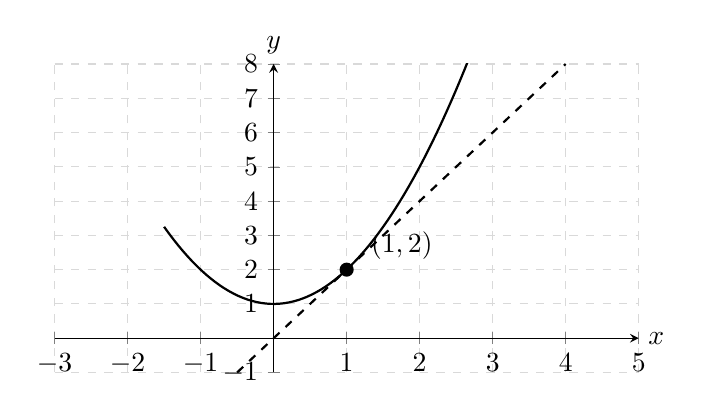
\begin{tikzpicture}
\begin{axis}[
  axis lines=middle,
  xlabel={$x$},
  ylabel={$y$},
  grid=both,
  grid style={dashed, gray!30},
  xmin=-3, xmax=5,
  ymin=-1, ymax=8,
  xtick={-3,-2,...,5},
  ytick={-1,0,...,8},
  width=9cm,
  height=5.5cm,
  every axis x label/.style={at={(ticklabel* cs:1.0)}, anchor=west},
  every axis y label/.style={at={(ticklabel* cs:1.0)}, anchor=south},
]
  \addplot[thick, domain=-1.5:3.5, samples=80] {x^2 + 1};
  \addplot[thick, dashed, domain=-0.5:4] {2*x};
  \node[circle, fill, inner sep=1.8pt] at (axis cs:1,2) {};
  \node[anchor=south west] at (axis cs:1.2,2) {$(1, 2)$};
\end{axis}
\end{tikzpicture}
\end{center}

%--- Problem 4: Graph interpretation with discriminant [6 marks] ---
\item[4.] [Maximum mark: 6]

The diagram shows the graph of $f(x) = -(x - 3)^2 + 4$.

\begin{enumerate}[itemsep=0.3cm]
  \item Vertex: $(3, 4)$ \hfill \textbf{(A1)}

  \item $f(x) = -(x^2 - 6x + 9) + 4 = -x^2 + 6x - 9 + 4 = -x^2 + 6x - 5$ \hfill \textbf{(M1)(AG)}

  \item $-x^2 + 6x - 5 = 0 \implies x^2 - 6x + 5 = 0$ \hfill \textbf{(M1)}

  $(x - 1)(x - 5) = 0$, so $x = 1$ and $x = 5$ \hfill \textbf{(A1)}

  \item $\Delta = 6^2 - 4(1)(5) = 36 - 20 = 16 > 0$

  Since $\Delta > 0$, there are two distinct real roots,
  confirming two $x$-intercepts. \hfill \textbf{(A1)}
\end{enumerate}

\newpage

%--- Problem 5: Completing the square [6 marks] ---
\item[5.] [Maximum mark: 6]

Consider the function $f(x) = 2x^2 - 8x + 11$.

\begin{enumerate}[itemsep=0.3cm]
  \item $f(x) = 2(x^2 - 4x) + 11 = 2(x^2 - 4x + 4 - 4) + 11$ \hfill \textbf{(M1)}

  $= 2(x - 2)^2 - 8 + 11 = 2(x - 2)^2 + 3$ \hfill \textbf{(A1)}

  \item Vertex: $(2, 3)$ \hfill \textbf{(A1)}

  \item $\Delta = (-8)^2 - 4(2)(11) = 64 - 88 = -24 < 0$ \hfill \textbf{(M1)}

  Since $\Delta < 0$, the equation has no real solutions. \hfill \textbf{(AG)}

  \item Minimum value of $f(x)$ is $3$ (the $k$-value from vertex form). \hfill \textbf{(A1)}
\end{enumerate}

%--- Problem 6: Polynomial factoring [6 marks] ---
\item[6.] [Maximum mark: 6]

Let $p(x) = x^3 - 6x^2 + 11x - 6$.

\begin{enumerate}[itemsep=0.3cm]
  \item $p(1) = 1 - 6 + 11 - 6 = 0$ \hfill \textbf{(M1)}

  Since $p(1) = 0$, $(x - 1)$ is a factor by the factor theorem. \hfill \textbf{(R1)}

  \item By polynomial division (or inspection):

  $x^3 - 6x^2 + 11x - 6 = (x - 1)(x^2 - 5x + 6)$ \hfill \textbf{(M1)}

  $= (x - 1)(x - 2)(x - 3)$ \hfill \textbf{(A1)}

  \item Solutions: $x = 1$, $x = 2$, $x = 3$ \hfill \textbf{(A1)}

  \item Cubic curve crossing the $x$-axis at $x = 1, 2, 3$
  and the $y$-axis at $(0, -6)$. Positive leading coefficient
  gives the standard cubic shape ($-\infty$ to $+\infty$). \hfill \textbf{(A1)}
\end{enumerate}

\end{enumerate}
\end{document}
